\begin{question}
\noindent Triangle $T$ is drawn on the grid below.

\begin{center}
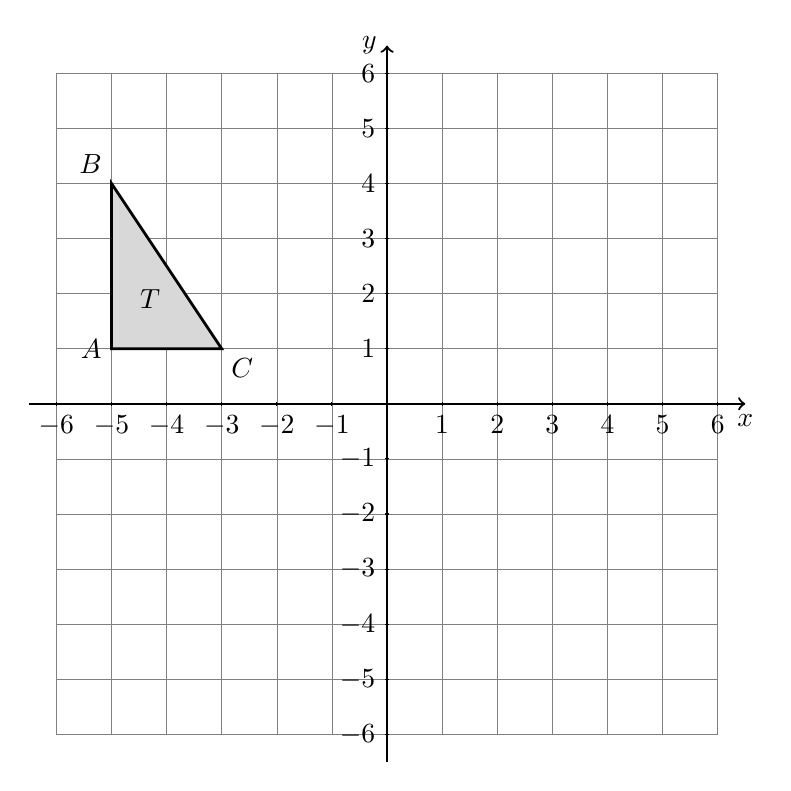
\begin{tikzpicture}[scale=0.7]
    % Define axis scale
    \def\axisLimit{6}

    \definecolor{borderColour}{HTML}{000000}
    \definecolor{fillColour}{HTML}{D8D8D8}

    % Draw grid
    \draw[step=1cm,gray,very thin] (-\axisLimit,-\axisLimit) grid (\axisLimit,\axisLimit);

    % Draw axes
    \draw[thick,->] (-\axisLimit-0.5,0) -- (\axisLimit+0.5,0) node[anchor=north] {$x$};
    \draw[thick,->] (0,-\axisLimit-0.5) -- (0,\axisLimit+0.5) node[anchor=east] {$y$};

    % Label x-axis and y-axis
    \foreach \x in {-6,-5,...,-1,1,2,...,6}
        \draw (\x cm,1pt) -- (\x cm,-1pt) node[anchor=north] {$\x$};
    \foreach \y in {-6,-5,...,-1,1,2,...,6}
        \draw (1pt,\y cm) -- (-1pt,\y cm) node[anchor=east] {$\y$};

    % Define coordinates for triangle T
    \coordinate (A) at (-5,1);
    \coordinate (B) at (-5,4);
    \coordinate (C) at (-3,1);

    % Draw triangle T
    \filldraw[fill=fillColour, draw=borderColour, line width=1pt] (A) -- (B) -- (C) -- cycle;

    % Labels
    \node[left] at (A) {$A$};
    \node[above left] at (B) {$B$};
    \node[below right] at (C) {$C$};
    \node at (-4.3,1.9) {$T$};

\end{tikzpicture}
\end{center}

\noindent Triangle $T$ is translated by the vector $\begin{pmatrix} 6 \\ -2 \end{pmatrix}$ to give triangle $T'$.

\noindent On the grid, draw and label triangle $T'$, and state the coordinates of the image of vertex $A$.

\vspace{5cm}

\begin{flushright}
    \answercoord{2}
\end{flushright}
\end{question}
